\documentclass{article}
\usepackage{tikz}
\usetikzlibrary{decorations.pathreplacing, calc}

\begin{document}

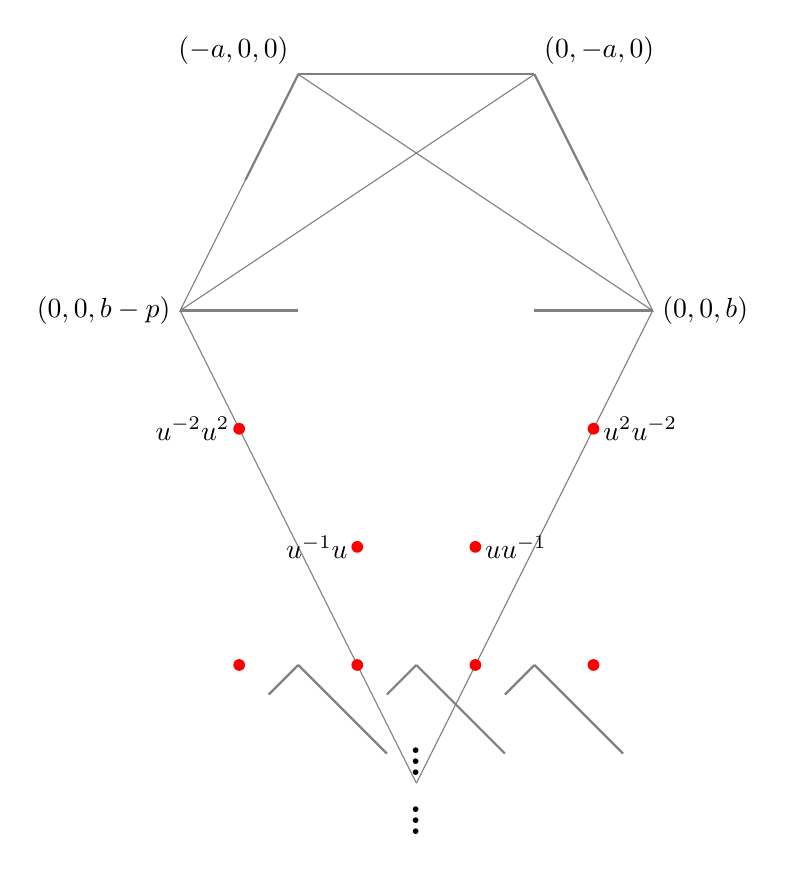
\begin{tikzpicture}[scale=1.5]
    % Define points
    \coordinate (O) at (0,0);
    \coordinate (A) at (-2,4);
    \coordinate (B) at (2,4);
    \coordinate (C) at (-1,6);
    \coordinate (D) at (1,6);
    
    % Draw lattice structure
    \draw[thin, gray] (O) -- (A); \draw[thin, gray] (O) -- (B);
    \draw[thin, gray] (A) -- (C) -- (D) -- cycle;
    \draw[thin, gray] (B) -- (C) -- (D) -- cycle;
    
    \draw[thick, gray] (C) -- ($(C)!1cm!(D)$);
    \draw[thick, gray] (D) -- ($(D)!1cm!(C)$);
    
    \draw[thick, gray] (C) -- ($(C)!1cm!(A)$);
    \draw[thick, gray] (D) -- ($(D)!1cm!(B)$);
    
    \draw[thick, gray] (A) -- ($(A)!1cm!(B)$);
    \draw[thick, gray] (B) -- ($(B)!1cm!(A)$);
    
    % Label points
    \node at (A) [left] {$(0,0,b-p)$};
    \node at (B) [right] {$(0,0,b)$};
    \node at (C) [above left] {$(-a,0,0)$};
    \node at (D) [above right] {$(0,-a,0)$};
    
    % Red nodes with labels
    \node at (0.5,2) [circle, fill=red, inner sep=1.5pt] {};
    \node at (0.5,2) [right] {$uu^{-1}$};
    
    \node at (-0.5,2) [circle, fill=red, inner sep=1.5pt] {};
    \node at (-0.5,2) [left] {$u^{-1}u$};
    
    \node at (-1.5,3) [circle, fill=red, inner sep=1.5pt] {};
    \node at (-1.5,3) [left] {$u^{-2}u^2$};
    
    \node at (1.5,3) [circle, fill=red, inner sep=1.5pt] {};
    \node at (1.5,3) [right] {$u^2u^{-2}$};
    
    % Points at the bottom
    \node at (-1.5,1) [circle, fill=red, inner sep=1.5pt] {};
    \node at (-0.5,1) [circle, fill=red, inner sep=1.5pt] {};
    \node at (0.5,1) [circle, fill=red, inner sep=1.5pt] {};
    \node at (1.5,1) [circle, fill=red, inner sep=1.5pt] {};
    
    \foreach \x in {-1,0,1} {
        \draw[thick, gray] (\x,1) -- (\x+0.75,0.25);
    }
    
    \foreach \x in {-1,0,1} {
        \draw[thick, gray] (\x,1) -- (\x-0.25,0.75);
    }
    
    \node at (0,-0.25) {\Huge$\vdots$};
    \node at (0,0.25) {\Huge$\vdots$};
\end{tikzpicture}

\end{document}